\section{Nowcasting GDP}
\label{chapter4_section3}



To obtain a preliminary view on the respective performances of the different model, a simple plot of the predictions can prove useful. On Figure \ref{fig_c4_s3_1}, each row represents a prediction horizon (1 quarter ahead or nowcast at the top, up to 4 quarters ahead at the bottom). Each column represents one class of models: nowcasting on the left, econometrics in the middle, and machine learning on the right. The actual GDP data which represents the prediction target is depicted by the black line. The other models are represented for each class by the green, orange and purple lines.

Taking an overall view on the picture, it seems that none of the models manages to capture very closely the dynamics of the data, whatever the prediction horizons. Most of them exhibit periods of good fit, and other periods where the link with the target data becomes quite loose.

\newpage

\begin{figure}[H]
\centering
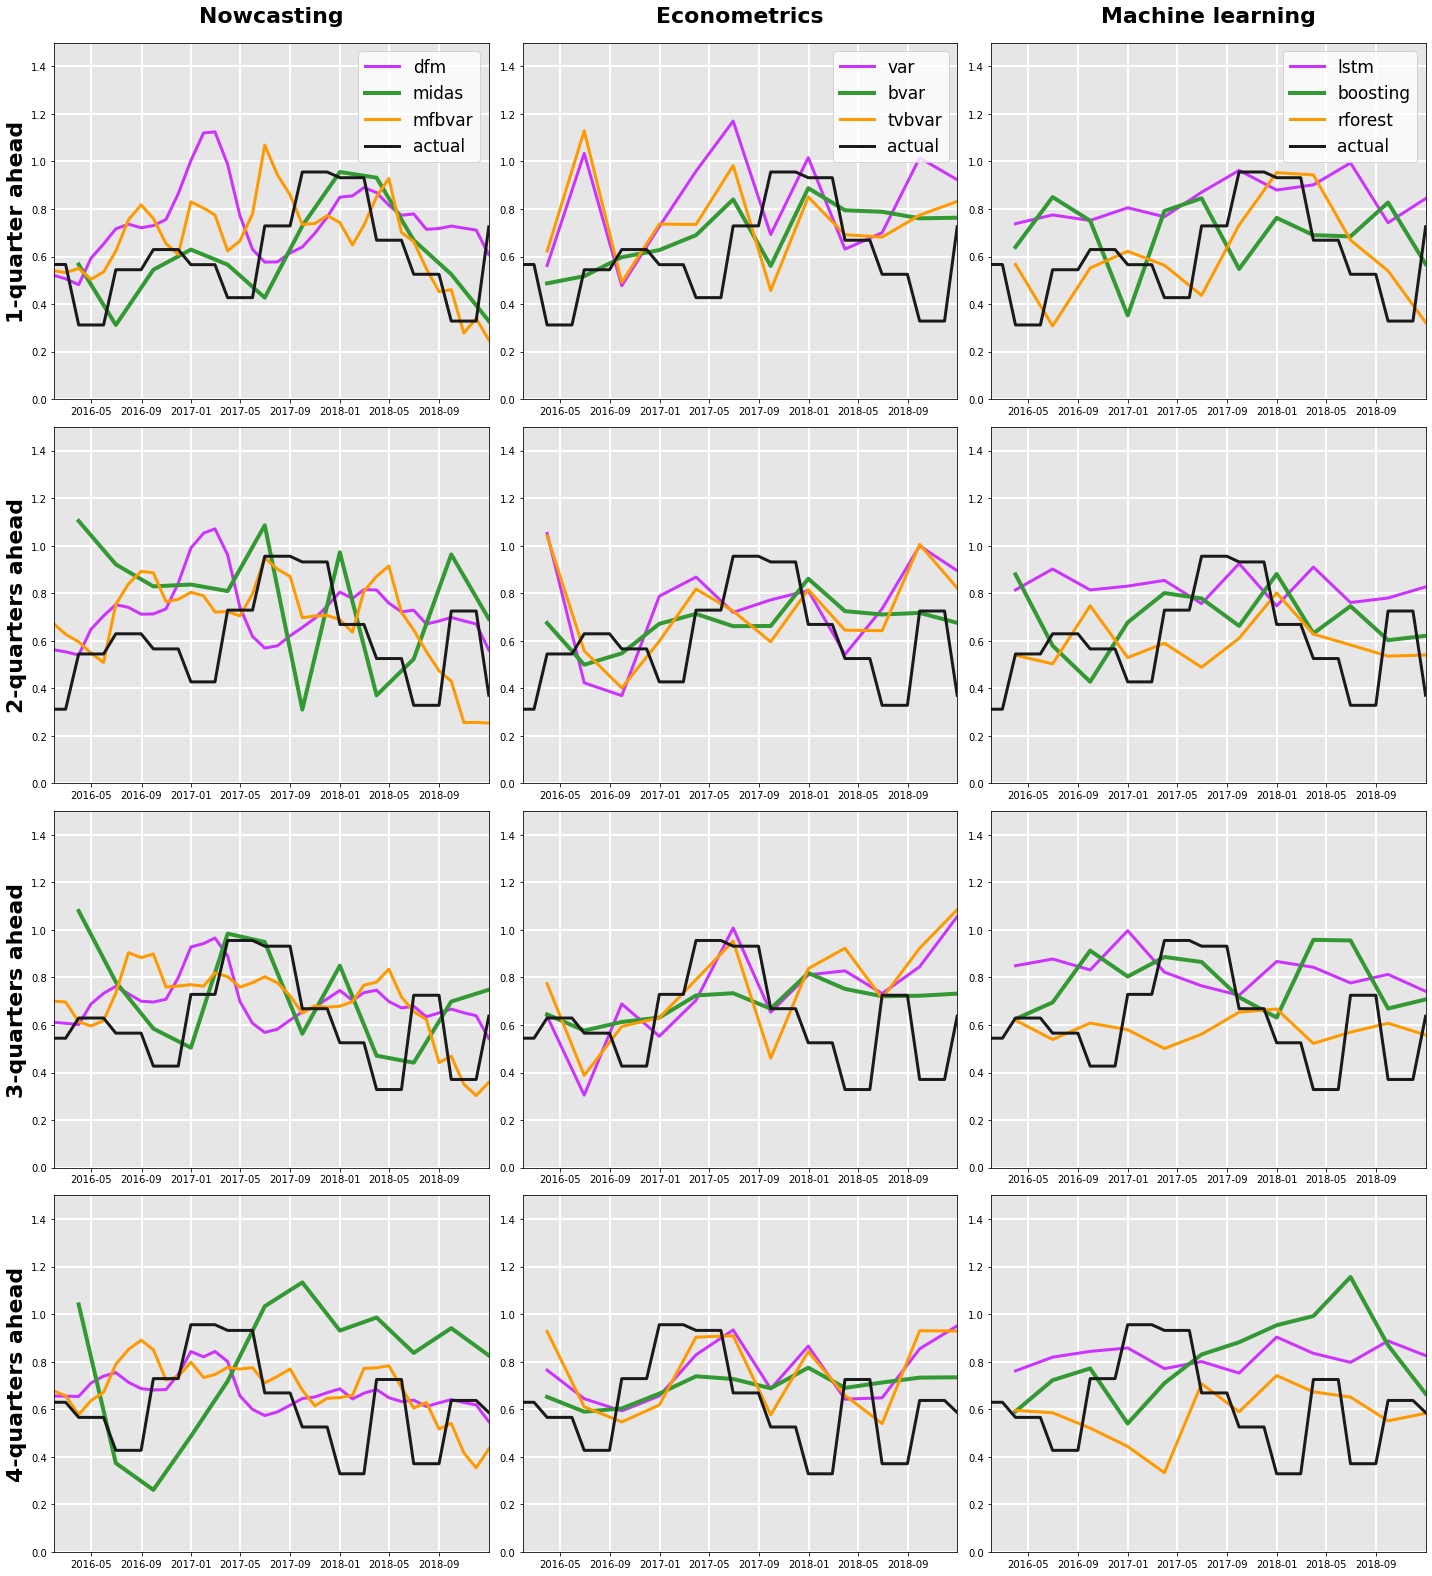
\includegraphics[scale=0.32]{images/predictions.png}
\caption{GDP predictions: all models, all prediction horizons}
\label{fig_c4_s3_1} \vspace{-6mm}
\end{figure}

Looking at the nowcasting models, the dynamic factor model seems to perform average overall. Its fit is never really close, save perhaps for the 3 quarters ahead horizon. The MIDAS regression seems to perform reasonably well at the nowcasting horizon, but exhibit a lag between the dynamics and the prediction. Its performances significantly degrade at longer horizons. The mixed frequency Bayesian VAR produces fair performances. At nowcast horizons, it shows average performance on the first half of the sample and good performance on the second half.

In terms of econometrics models, the picture looks fairly clear. Both the regular VAR and the time-varying BVAR displays large swings which keep them most of the time far from the target. This is probably the effect of overfitting for the former, and the the capture of artifical dynamc moves for the latter. The Bayesian VAR by contrast shows predictions of more moderate amplitudes, as a consequence of the Minnesota prior which generates a parsimonious model. Its predictions look overall closer to the target.

The machine learning models, finally, don't seem to perform very well. The boosting approach seems to produce large and short-lived oscillations revolving around the target. The random forest predictions are virtually similar to that produced by the MIDAS regression. These two models share the same features, so this only indicates that the parsimonious feature selection exerted by the random forest is quite equivalent to the parsimonious lag structure strategy of the standard MIDAS regression. In the end, the random forest suffers from the same quality and defaults as the MIDAS model: the predictions may look close to the actual values, but they actually always come with a lag. The LSTM, finally, produces smoother predictions. It is however clear that it is biased upward, resulting in poor predictions.

To confirm these intuitions formally, the average RMSE on the predictions of the forecasting exercise are reported in Table \ref{table_c4_s3_1}. For each prediction horizon (i.e. each column), the green entry represents the best predictor while the yellow entry marks the second best prediction. \vspace{2mm}

\begin{table}[H] \centering
\scalebox{0.8}{\setlength{\extrarowheight}{-0.4em} \begin{tabular}{@{} llcccc @{}}
\toprule[0.5mm]
& & 1 quarter ahead & 2 quarters ahead & 3 quarters ahead & 4 quarters ahead \\
\cmidrule{1-6}
\multirow{3}{*}{nowcasting} & dfm & 0,707 & 0,694 & 0,598 & \colorbox{coolgreen}{\phantom{aaaa} 0,443 \phantom{aaaa}} \\
& midas & 0,593 & 0,909 & 0,609 & 1,154 \\
& mfbvar & \colorbox{coolyellow}{\phantom{aaaa} 0,536 \phantom{aaaa}} & 0,613 & \colorbox{coolyellow}{\phantom{aaaa} 0,543 \phantom{aaaa}} & \colorbox{coolyellow}{\phantom{aaaa} 0,503 \phantom{aaaa}} \\
\cmidrule{1-6}
\multirow{3}{*}{econometrics} & var & 0,885 & 0,808 & 0,697 & 0,729 \\
& bvar & \colorbox{coolgreen}{\phantom{aaaa} 0,502 \phantom{aaaa}} & \colorbox{coolgreen}{\phantom{aaaa} 0,558 \phantom{aaaa}} & \colorbox{coolgreen}{\phantom{aaaa} 0,486 \phantom{aaaa}} & 0,547 \\
& tvbvar & 0,784 & 0,732 & 0,740 & 0,706 \\
\cmidrule{1-6}
\multirow{3}{*}{machine learning} & lstm & 0,712 & 0,747 & 0,769 & 0,745 \\
& random forest & 0,592 & \colorbox{coolyellow}{\phantom{aaaa} 0,566 \phantom{aaaa}} & 0,635 & 0,552 \\
& boosting & 0,605 & 0,568 & 0,594 & 0,548 \\
\cmidrule{1-6}
\multirow{4}{*}{benchmarks} & last value & 0,593 & 0,697 & 0,775 & 0,749 \\
& ridge var & 0,835 & 0,761 & 0,704 & 0,678 \\
& nowcasting.com & 0,668 & 0,679 & -- & -- \\
& bloomberg & 1,019 & -- & -- & -- \\
\bottomrule[0.5mm]
\end{tabular}}
\captionsetup{justification=centering}
\caption{\textbf{RMSE on GDP forecasts: all horizons}}
\label{table_c4_s3_1}
\end{table}

\newpage

A few conclusions stand. First, two models seem to dominate the whole exercise: the Bayesian VAR (as the best model), and the mixed frequency Bayesian VAR (as the second best model). The conclusion is very robust as the two models always produce the best performance, except in two cases (the random forest at 2 quarters ahead and the dynamic factor model at 4 quarters ahead) where their performance remains significantly better than most of their competitors. Also, their RMSE proves considerably lower than that of the other models, usually of the order of 20\% to 40\%, so their superiority is quite significant. These two models share a number of properties: they are linear models; they are trained on the small dataset; and they both benefit from a parsimonious representation due to the implementation of the Minnesota prior. This suggests that the behaviour of the data is best represented by a linear regime using only the features with the most explanatory power and only a limited number of parameters to define the dynamics.

The second conclusion is that the class of nowcasting models don't produce the best short term performance (except of course the mfbvar), even though they are built for this purpose . The dynamic factor model and the MIDAS regression achieve fair, but not excellent predictions, even though they make use of high frequency, monthly data to extract more information about the incoming quarterly release. One possible explanation is the overly simplistic formulation of these two models. Another explanation, possibly more convincing, is the dichotomy that exists within these models. On the one hand, the dynamics of the high frequency features is estimated on $T$ monthly observations. On the other hand, the predictive model of the low frequency GDP can still only be estimated on $T/3$ observations, due to the quarterly nature of the series. Apparently the reduced number of low frequency observations used to train the predictive model for GDP eventually anihilates the benefit of the larger high frequency sample.

The third conclusion is the incapacity of the machine learning models to produce very good predictions, save for the random forest at nowcast horizons. This in fact hardly surprising. These models are primarily designed to detect nonlinear behaviours, and are very data greedy. By contrast, the dataset of the exercise exhibit simple linear behaviours, and the dataset is quite short. The detected nonlinearities are probably the outcome of noisy processes rather than underlying dynamics, leading to overfitting and mediocre predictions. The same conclusion holds indeed for the tv-BVAR, typically intended to capture abrupt and nonlinear changes in the dynamics, which results here in poor predictions.

The final conclusion is that none of the benchmarks manage to beat the BVAR and the mf-BVAR. In particular, the professional forecasts propose by Bloomberg and Nowcasting.com are significantly worse than the predictions produced by the simple Bayesian VAR. In fact, the performance of the nowcasting.com predictions are quite similar to that of the dynamic factor model developed for the project, confirming the robustness of the conclusion. The Ridge VAR performs poorly at any horizon. Most likely, the blind regularization applied by the methodology cannot compete with the more selective regularization induced by the Minnesota prior. 

The simple predictor using the last known sample value performs surprisingly well at short horizon, beating most other models. Interstingly enough, the MIDAS regression and the random forest produce virtually similar performance. This is because these two models essentially replicate the last value for their nowcasts, as can be seen from Figure \ref{fig_c4_s3_1}. This trivial predictor may thus represent a good option, even though it is  possible to achieve better predictions than this simplistic strategy.

These results are not fully refined. Indeed, two models in the panel are estimated at the monthly frequency: the dynamic factor model and the mixed frequency Bayesian VAR, to which must be added the dynamic factor model of Nowcasting.com. Because these models are monthly, three forecasts are produced for a given quarter: three months before, two months before, and one month before the release. The timing of the prediction may matter: as more information normally yields more accurate forecasts, predictions closer to the release should be better than early forecasts. Table \ref{table_c4_s3_2} reports the average RMSE for the four models, distinguishing the different timings before release.

\begin{table}[H] \centering
\scalebox{0.8}{\setlength{\extrarowheight}{-0.4em} \begin{tabular}{@{} lccc @{}}
\toprule[0.5mm]
& 3 months before & 2 months before & 1 month before \\
\cmidrule{1-4}
dfm & 0,755 & 0,703 & 0,663 \\
mfbvar & \colorbox{coolyellow}{\phantom{aaaa} 0,659 \phantom{aaaa}} & \colorbox{coolyellow}{\phantom{aaaa} 0,504 \phantom{aaaa}} & \colorbox{coolgreen}{\phantom{aaaa} 0,444 \phantom{aaaa}} \\
nowcasting.com & 0,726 & 0,620 & 0,659 \\
\cmidrule{1-4}
bvar benchmark & \colorbox{coolgreen}{\phantom{aaaa} 0,502 \phantom{aaaa}} & \colorbox{coolgreen}{\phantom{aaaa} 0,502 \phantom{aaaa}} & \colorbox{coolyellow}{\phantom{aaaa} 0,502 \phantom{aaaa}} \\
\bottomrule[0.5mm]
\end{tabular}}
\captionsetup{justification=centering}
\caption{\textbf{RMSE on nowcasts 1, 2 and 3 months before release}}
\label{table_c4_s3_2}
\end{table}

The results confirm the previous conclusions. The Bayesian VAR remains the best model three months and two months before release. The difference between the Bayesian VAR and the mixed frequency Bayesian VAR becomes however fairly insignificant at the two month horizon. At one month before release, the mixed frequency BVAR becomes best, with a significant discrepancy with the performance of the standard Bayesian VAR. This makes sense: because the Bayesian VAR is quarterly, the quarter represents the unit of measurement. Thus, predicting one quarter ahead implies a one period ahead prediction, and the Bayesian VAR performs well. The mixed frequency BVAR on the other hand is a monthly model. Hence a one quarter ahead prediction may imply a prediction up to three periods ahead. At three months before, the prediction proves much less accurate. Two months before the release, the two predictions play virtually at par: even though the mf-BVAR must predict at two periods ahead against one period only for the BVAR, the larger training sample and the additional information obtained in-between compensate and result in similar prediction performance. At one month before release, the mf-BVAR overtakes the Bayesian VAR and becomes the best predictor.

The other predictors provide consistent results and produce better forecasts as the timing gets closer to the release and more information is included in the information set. The dynamic factor model (both for the project and the one proposed by Nowcasting.com) looks overall weak compared to the Bayesian VAR models.

Beyond the pure measurement error illustrated by the Root Mean Squared Error, it migh also be of interest to analyse the capacity of a model to predict the right direction of change in GDP growth. Ideally, a model should not only produce predictions close to actual values, but it should also be capable of capturing adequately the direction of evolution of a variable, in particular in financial applications. The percentage of correct direction predictions are reported in Table \ref{table_c4_s3_3}.

\begin{table}[H] \centering
\scalebox{0.8}{\setlength{\extrarowheight}{-0.4em} \begin{tabular}{@{} llcccc @{}}
\toprule[0.5mm]
& & 1 quarter ahead & 2 quarters ahead & 3 quarters ahead & 4 quarters ahead \\
\cmidrule{1-6}
\multirow{3}{*}{nowcasting} & dfm & 0.556 & \colorbox{coolyellow}{\phantom{aaaa} 0.722 \phantom{aaaa}} & \colorbox{coolyellow}{\phantom{aaaa} 0.778 \phantom{aaaa}} & \colorbox{coolgreen}{\phantom{aaaa} 0.917 \phantom{aaaa}} \\
& midas & 0.417 & 0.667 & 0.667 & 0.583 \\
& mfbvar & \colorbox{coolgreen}{\phantom{aaaa} 0.805 \phantom{aaaa}} & 0.694 & \colorbox{coolgreen}{\phantom{aaaa} 0.833 \phantom{aaaa}} & \colorbox{coolyellow}{\phantom{aaaa} 0.861 \phantom{aaaa}} \\
\cmidrule{1-6}
\multirow{3}{*}{econometrics} & var & 0.417 & 0.667 & 0.667 & \colorbox{coolgreen}{\phantom{aaaa} 0.917 \phantom{aaaa}} \\
& bvar & \colorbox{coolyellow}{\phantom{aaaa} 0.667 \phantom{aaaa}} & 0.667 & \colorbox{coolgreen}{\phantom{aaaa} 0.833 \phantom{aaaa}} & 0.833 \\
& tvbvar & 0.417 & \colorbox{coolgreen}{\phantom{aaaa} 0.75 \phantom{aaaa}} & \colorbox{coolgreen}{\phantom{aaaa} 0.833 \phantom{aaaa}} & 0.833 \\
\cmidrule{1-6}
\multirow{3}{*}{machine learning} & lstm & 0.583 & \colorbox{coolgreen}{\phantom{aaaa} 0.75 \phantom{aaaa}} & \colorbox{coolgreen}{\phantom{aaaa} 0.833 \phantom{aaaa}} & 0.583 \\
& random forest & 0.417 & \colorbox{coolgreen}{\phantom{aaaa} 0.75 \phantom{aaaa}} & 0.5 & 0.417 \\
& boosting & 0.583 & 0.583 & 0.75 & 0.167 \\
\bottomrule[0.5mm]
\end{tabular}}
\captionsetup{justification=centering}
\caption{\textbf{Percentage of correct direction predictions}}
\label{table_c4_s3_3}
\end{table}

At the nowcast horizon, the mixed frequency Bayesian VAR et the Bayesian VAR significantly dominate the other models. They represent, in fact, the only models that predict the correct direction of change more than two third of the times. The other models are either slitghly better than a random predictor, or below it like the MIDAS regression or the random forest. This is expected: because the MIDAS and random forest models are equivalent to the last value predictor at nowcast horizon, they miss the directional change most of the time, resulting in poor dorectional performance. 

At longer horizon, the dynamic factor model displays good performances overall, predicting the correct direction in more than 70\% of the cases. It is however (marginally) overperformed by other models like the tvbvar and the lstm, at the horizon of two and three quarters. It becomes the best model at the four quarter horizon. The VAR, random forest and boosting model produce overall poor performances. Eventually, which model is best to predict the direction beyond the nowcast horizon remains inconclusive.

As a conclusion to this section, it seems clear that two models dominate the nowcast exercise for GDP: the Bayesian VAR, and the mixed frequency Bayesian VAR. The two models are better than their competitors both in terms of forecast accuracy, and capacity to predict the correct direction of change. The standard Bayesian VAR performs best when the prediction is preduced one full quarter before the release. One month before release, higher frequency variables are updated and the mixed frequency BVAR becomes dominant. Which model is most suitable at the two month deadline remains ambiguous.




